Tasks can appear in different contexts. For example, we often use tasks to indicate a code region in shared and distributed memory programming models. However, this definition is loose and not clear to determine where is the task space and which is the task data or task input/output.\\

In task-based parallel programming, tasks are defined more consistently. We define a task by a code entry and its data. The data indicate input, output, or data region that a task can manipulate. When the input/output of a task is associated with other tasks, these tasks are dependent. Porting a normal application into a task-based one can help simplify the parallel execution such a well-expressed parallelism.\\

In terms of execution, a specific implementation of task-based programming models is considered as a library or a framework. This library attempts to separate parallel programs into a pool of tasks and a pool of computing resource units. The pool of computing resource units indicates threads within a process. These two pools imply two levels: application level and system level. From the application level, we can see task-based applications as a black box. From the system level, we can see task-based programming models as runtimes. The runtimes manage tasks and handle performance portability \cite{aumage2021taskportability}. Performance portability means:
\begin{itemize}
	\item Users can simplify parallel applications as tasks alongside their data.
	\item Users can quickly port parallel applications to new and different platforms.
	\item Users can be relaxed in terms of task scheduling, load balancing, and overlapping communication-computation at the side of task-based runtimes.
\end{itemize}

% Note: definition between framework, library, api
% 	+ library: a collection of code (e.g., functions, objects) to perform common tasks. It tends to be stable and bug free. Using appropriate libs can reduce the amount of code that needs for writting the program.
%		+ API (Application Programming Interface): provides some functionality which allows an application to access the available functionality. It exists at many levels including system, library, framework, program.
% 	+ Framework: is a collection of APIs designed to make building of application simpler.
%
%		-------------------
%		- Framework 			-
%		-------------------
%		- Library   			-
%		-------------------
%		- API       			-
%		-------------------

Based on the survey of Thoman et al. \cite{thoman2018taxonomy}, we summarize the main characteristics for classifying task-based parallel programming runtimes. These characteristics refer to application programming interfaces (API) in a given task-based runtime, which can be developed like a library, a language extension, or a language. The classification has four aspects: Architecture, Task System, Task Management, and Engineering. Table \ref{tab:taskbased-apis} summarizes this classification associated with various task-based runtimes and libraries today.

\begin{itemize}
	\item Architecture: highlights the target systems or computer architectures. In detail, the related factors of architecture are further divided into three components.
		\begin{itemize}
			\item Communication model: shared memory, message passing, and an abstraction model called global address space, which is created as a shared memory model for distributed memory systems. These terms are denoted by $smem$, $msg$, $gas$, respecively in Table \ref{tab:taskbased-apis}.
			\item Distributed memory system: the compatibility with distributed memory is explicit, implicit, or no support. The terms of ``implicit'', ``explicit'', ``no support'' are denoted by $i$, $e$, \xmark, respectively.
			\item Heterogeneity: indicates whether tasks can be ported to accelerators or not. The classification is also denoted by explicit, implicit, or no support with $i$, $e$, and \xmark, respectively.
		\end{itemize}
		
	\item Task System: shows how tasks are built and simplified with or without dependencies. The main factors are structure and task partitioning. Furthermore, we can also classify them by result handling and task cancellation.
		\begin{itemize}
			\item Graph structure: the possibilities of representing task dependency include tree ($tree$), acyclic graph ($dag$), arbitrary graph ($graph$), or no dependency.
			\item Task partitioning: indicates whether a task is atomic ($atom$ or \cmark) or can be divisible ($div$ or \xmark).
		\end{itemize}
	
	\item Task Management: is related to task assignment and resource management. Moreover, this characteristic focuses on how tasks are supported for resilience as well as debugging.
		\begin{itemize}
			\item Worker management: indicates whether the worker threads/processes (which execute tasks) are maintained ``explicit'' by users or ``implicit'' (automatically) by the environment.
			\item Work mapping: describes the strategy that tasks are assigned to computing resource units. The possibilities include ``explicit'' mapping or ``implicit'' mapping.
		\end{itemize}
		
	\item Engineering: shows how a task-based programming interface is used or implemented, such as a library ($lib.$), a language extension ($ext.$), or a language ($lang.$).
\end{itemize}

\begin{table}[t]
\centering
\scalebox{0.9}{
\begin{tabular}{|l|lll|ll|ll|l|}
\hline
\multirow{2}{*}{\textbf{APIs}} & \multicolumn{3}{c|}{\textbf{Architecture}} & \multicolumn{2}{c|}{\textbf{Task System}} & \multicolumn{2}{c|}{\textbf{Task Management}} & \multicolumn{1}{c|}{\multirow{2}{*}{\textbf{Engineering}}} \\ \cline{2-8}
		& \multicolumn{1}{l|}{\rotatebox{270}{Communication model }} & \multicolumn{1}{l|}{\rotatebox{270}{Distributed memory}} & \rotatebox{270}{Heterogeneity} & \multicolumn{1}{l|}{\rotatebox{270}{Graph structure}} & \rotatebox{270}{Task partitioning} & \multicolumn{1}{l|}{\rotatebox{270}{Worker management}} & \rotatebox{270}{Work mapping} & \multicolumn{1}{c|}{}                             \\ \hline
	C++ STL \cite{kormanyos2015} & \multicolumn{1}{l|}{smem} & \multicolumn{1}{l|}{\xmark} & \xmark & \multicolumn{1}{l|}{dag} & \xmark & \multicolumn{1}{l|}{\textbf{i}} & \textbf{i/e} & lib. \\ \hline
	TBB \cite{willhalm2008putting} & \multicolumn{1}{l|}{smem} & \multicolumn{1}{l|}{\xmark} & \xmark & \multicolumn{1}{l|}{tree} & \xmark & \multicolumn{1}{l|}{\textbf{i}} & \textbf{i} & lib. \\ \hline
	HPX \cite{kaiser2014hpx} & \multicolumn{1}{l|}{gas} & \multicolumn{1}{l|}{i} & \textbf{e} & \multicolumn{1}{l|}{dag} & \cmark & \multicolumn{1}{l|}{\textbf{i/e}} & \textbf{i/e} & lib. \\ \hline
	Legion \cite{bauer2014legion} & \multicolumn{1}{l|}{gas} & \multicolumn{1}{l|}{i} & \textbf{e} & \multicolumn{1}{l|}{tree} & \cmark & \multicolumn{1}{l|}{\textbf{i}} & \textbf{i/e} & lib. \\ \hline
	PaRSEC \cite{hoque2017dynamic} & \multicolumn{1}{l|}{msg} & \multicolumn{1}{l|}{e} & \textbf{e} & \multicolumn{1}{l|}{dag} & \xmark & \multicolumn{1}{l|}{\textbf{i}} & \textbf{i/e} & lib. \\ \hline
	Chameleon \cite{Klinkenberg2020ChameleonReactLB} & \multicolumn{1}{l|}{msg} & \multicolumn{1}{l|}{e} & \xmark & \multicolumn{1}{l|}{dag} & \cmark & \multicolumn{1}{l|}{\textbf{e}} & \textbf{i/e} & lib. \\ \hline
	Taskflow \cite{huang2020cpp} & \multicolumn{1}{l|}{smem} & \multicolumn{1}{l|}{\xmark} & \textbf{e} & \multicolumn{1}{l|}{dag} & \cmark & \multicolumn{1}{l|}{\textbf{i/e}} & \textbf{i/e} & lib. \\ \hline
	OpenMP \cite{ayguade2008design} & \multicolumn{1}{l|}{smem} & \multicolumn{1}{l|}{\xmark} & \textbf{i} & \multicolumn{1}{l|}{dag} & \xmark & \multicolumn{1}{l|}{\textbf{e}} & \textbf{i} & ext. \\ \hline
	Charm++ \cite{acun2014parallel} & \multicolumn{1}{l|}{gas} & \multicolumn{1}{l|}{\textbf{i}} & \textbf{e} & \multicolumn{1}{l|}{dag} & \cmark & \multicolumn{1}{l|}{\textbf{i}} & \textbf{i/e} & ext. \\ \hline 
	OmpSs \cite{duran2011ompss} & \multicolumn{1}{l|}{smem} & \multicolumn{1}{l|}{\xmark} & \textbf{i} & \multicolumn{1}{l|}{dag} & \xmark & \multicolumn{1}{l|}{\textbf{i}} & \textbf{i} & ext. \\ \hline
	StarPU \cite{augonnet2011starpu} & \multicolumn{1}{l|}{smem} & \multicolumn{1}{l|}{\textbf{e}} & \textbf{e} & \multicolumn{1}{l|}{dag} & \cmark & \multicolumn{1}{l|}{\textbf{i}} & \textbf{i/e} & ext. \\ \hline
	Cilk Plus \cite{robison2012cilk} & \multicolumn{1}{l|}{smem} & \multicolumn{1}{l|}{\xmark} & \xmark & \multicolumn{1}{l|}{tree} & \xmark & \multicolumn{1}{l|}{\textbf{i}} & \textbf{i} & lang. \\ \hline
	X10 \cite{chrles2005x10} & \multicolumn{1}{l|}{gas} & \multicolumn{1}{l|}{\textbf{i}} & \textbf{i} & \multicolumn{1}{l|}{dag} & \cmark & \multicolumn{1}{l|}{\textbf{i}} & \textbf{i/e} & lang. \\ \hline
\end{tabular}}
\caption{An overview of the programming interface characteristics in various task-based parallel programming runtimes.}
\label{tab:taskbased-apis}
\end{table}

% Some relevant issues researched in task-based models might be listed as follows.
%\begin{itemize}
%	\item Continue to improve data locality decisions with more expressive abstractions of tasking.
%	\item Attempt to extend low-level resource management in HPC systems.
%	\item Relax application porting in more realistic use cases.
%	\item Support interoperability and proactive directions in scheduling and balancing tasks/loads.
%\end{itemize}

\clearpage

% ------------------------------------
% About task-based parallel applications
% ------------------------------------

\begin{figure}[t]
	\centering
	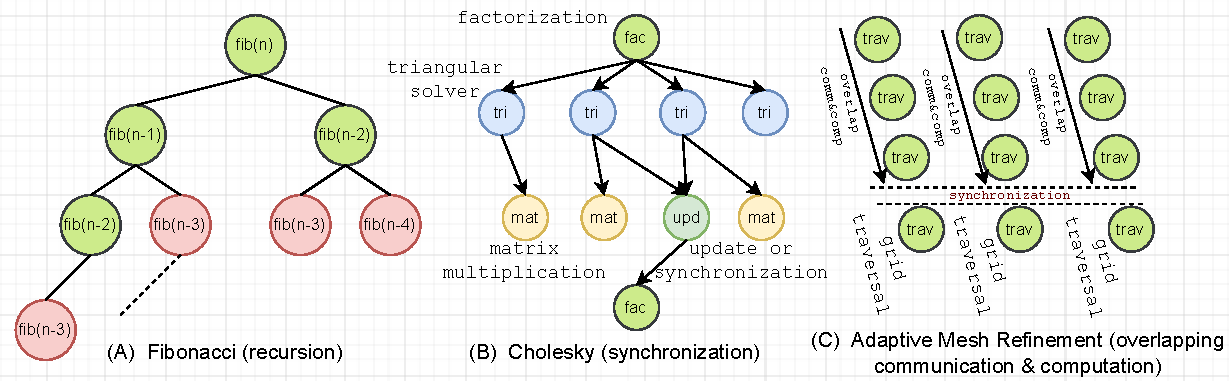
\includegraphics[scale=0.725]{./pictures/preliminaries/preli_task-based_app_usecases.pdf}
	\caption{Three examples illustrated as the three use cases of task-based parallel applications.}
	\label{fig:preli_taskbased_apps}
\end{figure}

\noindent There are three common use cases for porting an application to a task-based parallel application. They are known as recursion, complex synchronization, overlapping computation and communication for numerical simulations. These three use cases are illustrated in Figure \ref{fig:preli_taskbased_apps}, including (A) Fibonacci, (B) Cholesky factorization, and (C) Adaptive Mesh Refinement.\\

The task-based version of Fibonacci defines tasks by its compute function (named \texttt{fib(n)}). The input data of tasks is an integer number. All tasks are generated recursively, tasks nested in another task. Using task-based parallel programming, we can facilitate the parallelism in Fibonacci with cut-off strategies as shown in Figure \ref{fig:preli_taskbased_apps} (A).\\

For Cholesky factorization, the difficulty is complex synchronization patterns. Porting Cholesky to a task-based parallel version can improve composability and clarify synchronization patterns. As shown in Figure \ref{fig:preli_taskbased_apps} (B), the program behavior is broken into separate tasks, such as computing factorization (\texttt{fac}), triangular solver (\texttt{tri}), matrix multiplication (\texttt{mat}), update (\texttt{upd}) as well as synchronization.\\

The rest is an example of Adaptive Mesh Refinement shown in Figure \ref{fig:preli_taskbased_apps} (C). It is known as a typical approach of numerical simulations in HPC. Here, tasks are defined by the function of traversing grid/mesh cells (denoted by \texttt{trav}). These tasks are independent, and their input data depends on the constraint parameters of simulation contexts, e.g., earthquake, tsunami. Executing Adaptive Mesh Refinement comprises multiple computation phases interwoven with synchronization phases, also called iterative execution. When running in distributed memory systems, each node executes an assigned part of the given grid. Therefore, there might be communication for exchanging grid information to compute the tasks. Using task-based programming, communication and computation can easily overlap. Especially the isolation between a pool of tasks and a pool of resources helps facilitate a dedicated communication thread by exchanging information during computation. Furthermore, Prat et al. \cite{prat2018taskbasedmdsim} also show the efficiency of task-based parallelism with another example, molecular dynamics (MD) simulations. Their MD implementation is $4.7\times$ faster than the state-of-the-art implementations (LAMMPS \cite{lammps2008mdsim}).\\

\noindent Task-based parallel runtimes help to simplify parallel programming. It is easier to manage tasks and control resources by separate pools. This offers an advantage for solving dynamic load balancing in distributed memory systems. The following section details how load balancing is formulated in task-based parallel applications and related work. 
